\chapter{Weryfikacja punktu pracy}
\label{zad1}

\section{Opis postępowania}
\label{zad1_opis}
W celu sprawdzenia poprawności wartości sygnałów $u$, $y$ oraz $z$ pobudzono obiekt sterowaniem
o wartości $u = \num{0.0}$, zakłóceniem $z = \num{0.0}$ i sprawdzeniu czy stabilizuje się on w punkcjie pracy  $y = \num{0.0}$. Do symulacji wyjscia obiektu użyto udostępnionej funkcji 
\verb+symulacja_obiektu4y.+ Do testów napisano skrypt \verb+Zad1.m. + Wyniki przedstawiono poniżej.

\section{Wyniki}
\label{zad1_wyniki}
Zgodnie z przewidywaniami wyjscie obiektu ustaliło się na wartości $y= \num{0.0}$. Punkt pracy ustalony jest więc poprawnie.
\begin{figure}[tb]
	\centering
	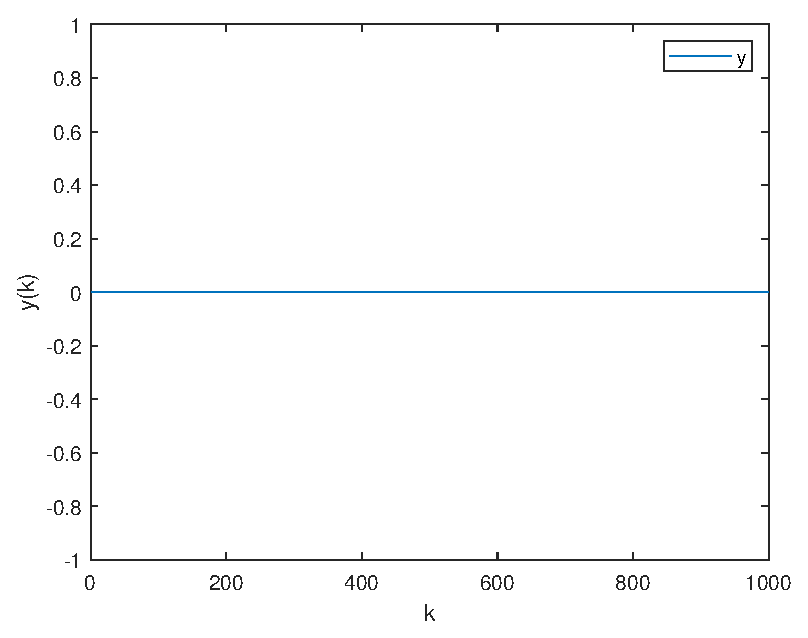
\includegraphics[scale=1]{Rys/punkt_pracy.eps}
	%\includegraphics[scale=1]{rysunki/zapisz_pdf/symulacje11}
	\caption{Odpowiedź obiektu na sterowaniei $u=\num{0.0}$ i zakłócenie $z = \num{0.0}$}
\end{figure}